\section{Introduction}
Despite the ubiquity, capacity and apparent efficacy, modern communication systems are wasteful, inefficient and in need of reform. Most of the bits of data collected by our sensing systems are unessential, and only serve to necessitate data compression wasting computation time before transmission. For example, people regularly use a camera with a resolution of several megapixels only to upload a file of a few kilobytes to Facebook. Devices are unable to make dynamic decisions about how to transmit this data, leading to both spectral exhaustion on some frequencies whilst much of the available radio spectrum lies fallow. 

This project addresses these issues, by reviewing a novel acquisition and decompression framework for data: a way in which we need only sense the most informative bits of data. This framework is then applied to the problem of sensing spectral opportunities dynamically, to make better use of available spectrum. 

The key uniting both these applications is that data and spectra are \textit{sparse}: that is they have a representations which are 'smaller' than their respective dimension. For example, images and audio can be compressed into file formats much smaller than when initially recorded (compare the relative sizes of bitmap and JPEG images).

The sole focus of this research is to use the sparsity of the spectrum to uncover transmission opportunities, allowing better use of spectrum more generally. 

We are motivated by the need to send more data over wireless networks, whilst at the same time having a constrained frequency set over which to transmit this information. This issue could be alleviated by users dynamically allocating spectrum on a per-transmission basis: without the ability to gain knowledge of spectral conditions this can never become a reality however. 

The requirement for increasing bandwidth isn't just a pressing issue for today: in the next decade it is forecast that network operators will need to provide for three-orders of magnitude (1000 times) more capacity. Demand is continually outstripping supply - motivated by the ubiquity of smart-phones, and the consumers appetites for media. 

At the same time as this demand for ever more data, there is an increasing scarcity of radio spectrum over which to transmit. New frequencies are rarely cleared for commercial purposes, and when they are they go for high prices.  A decade ago the UK auction for 3g spectrum licenses raised an estimated £22.4 billion \cite{Ukmobil} for the UK treasury, indicating the seriousness of the market players requirements for new spectrum. The recent 4g spectrum auction raised £2.3 billion \cite{BBC News}- with initial networks being rolled out by the end of 2013.

\begin{figure*}[h]
\centering
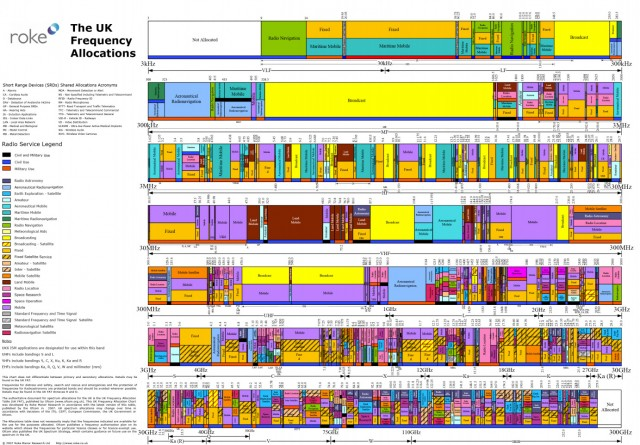
\includegraphics[height = 7 cm]{uk-spectrum-allocation-chart1-640x445.jpg}
\caption{A digram of current Spectral allocation \cite{Strategy2013}}
\label{spectrumalloc}
\end{figure*}

However, a closer inspection of the frequency allocation suggests this scarcity is artificial, it's more a product of regulatory oversight over time. As the constraints on spectrum requirement became more complex, so did the solutions to that problem - at the cost of leaving much of the spectrum idle for most of the time. 

For example: much of the spectrum is allocated to TV broadcast, radio broadcast and mobile. However, if we look closer, the allocations aren't even for specific companies - they're simply categories. Within these, OFCOM may have many licensees within each category.

Also interesting to note is how much frequency the Government allocates to itself (the red bar underneath the blocks indicates Government use). Compare this to the actual utilisation of spectrum: much of it is not used at all. Figure \ref{frequtil} shows a snapshot of frequency utilisation in three diverse locations in the UK over te radio specturm, note that many frequencies are not utilised (coloured blue) whilst others have significant activity (coloured yellow). Note that the plot for Southwark (central London) is barely different from Braddock - a rural area. 

\begin{figure*}[h]
\centering
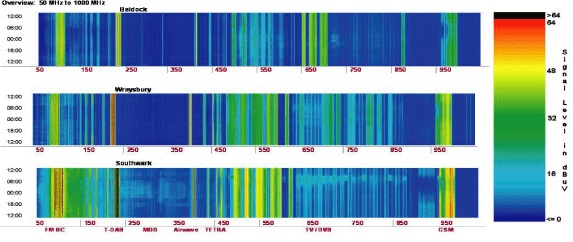
\includegraphics[height = 7 cm, width=0.5\textwidth]{cr2.jpg}
\caption{A snapshot of frequency utilisation in various areas: many frequencies are not used at all, whilst there is significant activity on others \cite{Burbidge2007}}
\label{frequtil}
\end{figure*}

How do we then go about solving this issue - how can we obtain the most significant bits of information from our sensing mechanism, whilst obviating the need to compress the data once we are done? How do we dynamically assign spectrum? The work of Candes, Tao \cite{Candes2006} and Donoho \cite{Donoho2006}, has shown that instead of measuring the information we require directly (and then compressing it), we can measure 'holographic' and non-linear random projections between our measurement space and the space where our data is sparse. This requires only the knowledge that the signal is compressible via some transform - both the acquisition protocol and the reconstruction algorithm are agnostic to the type of signal. What is surprising is that the sampling kernels are fixed independently of the signal, are non-adaptive and these projections are sufficient to reconstruct the signal - as if we had an Oracle to tell us where the non-zero components of our signal are. 

This work has had a large impact in medical imaging since it's inception: for example, it's now possible to take an image of a patient's heart within a single breath, as well as dynamic imaging of the heart (\cite{Donoho} figures 7 and 9).

Modern digital signal processing techniques (such as modulation techniques) are far more spectrally efficient than their historic analogue counterparts, which has in part contributed to the spectrum crisis. All this is changing though: from the beginning of 2013 all TV in the UK will transmitted digitally. Historically, television in the UK was broadcast using analogue signals requiring 32 multiplexes. Digital TV requires 6 multiplexes, on the other hand. 

This freeing up of TV frequencies represents an opportunity: these frequencies have good propagation characteristics (they suffer less with free space path loss relative to higher frequencies), whilst sill providing good bandwidth for data transmission. These TV frequencies are being opened up to civilian and  commercial users: spectral holes will be able to be exploited opportunistically by devices, so long as they don't interfere with the reception of TV. Historically, this is the single largest gift of new spectrum, and because there is no requirement for licensing this spectrum is free.

\begin{wrapfigure}{r}{0.5\textwidth}
\centering
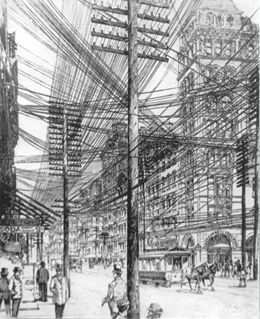
\includegraphics[width=0.48\textwidth, height = 7cm]{cablesnewyork.jpg}
\caption{A picture of early 20th century New York: Bandwidth has always been an issue}
\label{newyork}
\end{wrapfigure}

As with all technological innovations, this will not only improve existing infrastructure but also new classes of devices to transmit, for instance; applications such as passive sensor networks) which only need spectrum intermittently to transmit monitoring results), inter-vehicle communication for real time traffic monitoring and wireless internet at broadband data rates have all been proposed.

Despite all of this hype, dynamic spectrum access won't become a reality unless spectral holes can be robustly detected. The requirement that secondary users exploit the new spectrum politely, without interference to primary user makes spectrum sensing essential to TV white-space (TVWS) technologies. The realisation of any Cognitive Radio standard (such as IEEE 802.22), requires the co-existence of primary (TV users) and secondary (everybody else who wants to use TVWS spectrum) users of the frequency spectrum to ensure proper interference mitigation and appropriate network behaviour. 

Users of TVWS (Cognitive Radios) must sense whether spectrum is available, and must be able to detect very weak primary user signals. Furthermore they must sense over a wide bandwidth (due to the amount of TVWS spectrum proposed), which challenges traditional Nyquist sampling techniques, because the sampling rates required are not technically feasible with current RF or Analogue-to-Digital conversion technology.

Sensing should enable devices to detect the presence of TV signals in a band and provide smart and adaptive (and possibly distributed) solutions to band identification.

Spectrum sensing should involve:

\begin{enumerate}
\item Sensing to detect white spaces.
\item Co-existence with similar devices.
\item Frequency monitoring of other devices.
\item Interference management. 
\item Spectrum mobility and transmission power control when needed.
\end{enumerate}

As described earlier, the available spectrum is highly underutilised, and can be thought of as a collection of narrowband transmissions over a wideband channel. As such, the spectrum we're sensing is sparse. This makes it an ideal candidate for sparse recovery techniques such as Compressive Sensing.  

The report is divided into three chapters: the remainder of this chapter describes methods for sensing narrowband signals (i.e. channels where the frequency response is approximately flat, and where the bandwidth is smaller than the coherence bandwidth of the channel), and the limitations of these are highlighted for the problem of sensing spectrum for Cognitive Radios. 

Classical and Compressive Sensing are then contrasted, including the main ideas such as incoherence and the Restricted Isometry Property, and illustrating the number of samples required for full reconstruction.   Somme approaches to solving the optimisation problems posed by the new framework are also discussed.

Chapter 2 introduces Group Testing, and covers new work which has been accepted for publication at Allerton 2014. After some preliminary remarks the Capacity of a Group Testing problem is defined. Then, previous work on variations of an algorithm by Hwang are discussed, including upper and lower bounds on Capacity. Finally, a new algorithm is presented along with an analysis of the average number of tests the algorithm will execute.

The focus of Chapter 3 is again compressive sensing, this time in a distributed setting - given a connected network of nodes, how can we organise sensing to reconstruct a wideband signal? The chapter begins by discussing various signal models in the literature, and justifies the use of a single model. Then the sensing model is presented as a multinode extension of the Modulated Wideband Converter (\cite{Mishali2010}). There follows an extended discussion of constrained convex optimisation, and an introduction to the Alternating Direction Method of Multipliers. Finally, how to sense the requisite signals and use a distributed setup to solve the system is explained. Some tentative results of simulations are also presented.

\section{Narrowband Spectrum Sensing}

The problem of spectrum sensing is to decide whether a particular band is available, or not \cite{Y}. That is, we wish to discriminate between the following two hypotheses:

\begin{equation}
H_{0}: y\left[n\right] = w\left[n\right] \text{, n} =  1 \ldots N 
\end{equation}
\label{h1}

\begin{equation}
H_{1}: y\left[n \right] = x\left[n\right] + w\left[n\right] \text{, n} =  1 \ldots N 
\end{equation}
\label{h2}

Where \(x\) is the primary users signal, having a specific structure which stems from modern coding and modulation techniques, \(w\) is additive white Gaussian noise and \(y\) is the received signal.

To decide whether the observations \(\textbf{y}\) were generated under \(\textit{H}_{0}\) or \(\textit{H}_{1}\) is accomplished by forming a test statistic \(\Gamma\left(y\right)\) and then comparing this statistic with a predefined threshold \(\lambda\). Both classical methods, where the hypotheses are assumed to be deterministically true and the goal is to minimise the false detection probability, and Bayesian methods, where it is assumed that the source selects the true hypothesis at random according to some prior probabilities, agree that the test statistic should be likelihood ratio:

\begin{equation}
\Gamma\left(\textbf{y}\right) = \frac{p\left(\textbf{y}\mid H_0\right)}{p\left(\textbf{y}\mid H_1\right)}
\end{equation}

The performance of a detector is quantified in terms of the probability of detection

\begin{equation}
P_{D} = Pr\left( \Gamma\left(\textbf{y}\right) > \lambda \mid H_1\right)
\end{equation}

and the probability of false alarm 

\begin{equation}
P_{FA} = Pr\left( \Gamma\left(\textbf{y}\right) > \lambda \mid H_0\right)
\end{equation}

By varying \(\lambda\) the operating point of a detector can be chosen anywhere along its receiver operating characteristics curve.

There are several proposed spectrum sensing methods that enable cognitive radios identify bands and perform dynamic frequency selection. Some of the common (narrowband) spectrum sensing techniques are described below.

\subsubsection{Energy Detection}
This is a common method for the detection of unknown signals in noise, due to low computational and implementation complexity. This method is quite generic as receivers need no knowledge of the primary users signal. 

A typical method would be a bandpass filter with a centre frequency \(f_{s}\) and a bandwidth \(W\). This is followed by a squaring device to measure the received energy and an integrator to determine the observation interval. Finally the output of the integrator is compared with a threshold to determine the presence of a signal. This threshold is determined based upon the noise variance of the channel. I.e. we have a decision metric of the following form:

\begin{equation}
M = \sum_{n=0}^N |y\left[n\right]|^2
\end{equation}

Assuming that the signal is a zero mean AWGN variable as well, we can derive expressions for the metric, the detection probability and the false alarm probability:

\begin{equation}
 M =
  \begin{cases}
   \frac{\sigma_w^2}{2} & H_0 \\
   \frac{\sigma_w^2 + \sigma_s^2}{2} & H_1
  \end{cases}
\end{equation}

\begin{equation}
P_D = 1 - \Gamma\left(1, \frac{\lambda}{1 + \frac{ \sigma_2^2 }{ \sigma_w^2 } } \right)
\end{equation}

\begin{equation}
P_FA = 1 - \Gamma\left(1, \frac{\lambda}{\sigma_w^2} \right)
\end{equation}

Where \( \Gamma\left(1,x\right)\) is the incomplete gamma function. From these equations it's clear to see that the performance of energy detection based sensing faces challenges at low SNR values. See (REF) figure 3 for curves quantifying the performance. Also energy detectors perform poorly under extreme fading conditions as they are unable to distinguish primary users and noise. Further this type of detector is not efficient at detecting spread spectrum signals. 

Similarly because the threshold used to make the decision is based on the noise variance \(\sigma_w^2\), any error in the noise power estimation can cause significant performance loss. Various algorithms have been proposed to estimate this variance adaptively. See \cite{Yucek2009} for more details.

\subsubsection{Cyclostationary Feature Detection}
Because the signals used in practical communication systems contain distinctive features that can be exploited for detection, it is possible to achieve a detection performance which substantially surpasses the energy detector. This is in contrast to the predictions of information theory where maximum entropy signals will be statistically white and Gaussian (if this were the case, then we could do no better than the energy detector). More importantly, known signal features can be exploited to estimate unknown parameters such as noise power. 

Examples of well known patterns include pilot signals and spreading sequences. Other examples include preambles and midambles: known sequences transmitted before and in the middle of each slot, respectively. Others include redundancy added by coding, modulation and burst formatting used by the transmitter. 

This method exploits cyclostationary features of received signals: man made periodicity in the signal (for example symbol rate, chip rate, cyclic prefix etc) or its statistics - mean, autocorrelation. A cyclic correlation function is used instead of PSD (or autocorrelation sequence) for detecting signals present in a given spectrum. This is able to differentiate noise from primary users signals since noise is wide-sense stationary with no correlation but modulated signals are cyclostationary due to the redundancy of signal correlations. 

For clarity, the random processes encountered by a cognitive radio will have a period in both expectation and autocorrelation:

\begin{equation}
\mathbb{E}\left(t\right) = \mathbb{E}\left(t + mT\right) = \mathbb{E}\left[x\left(t\right)\right]
\end{equation}

\begin{equation}
\mathbb{R}\left(t, \tau\right) = \mathbb{R}\left(t + mT, \tau\right) = \mathbb{E}\left[x\left(t\right)\conjugate{x\left(t_+\tau\right)}\right]
\end{equation}

where \(t\) is time, \(\tau\) is the autocorrelation lag, \(x\left(t\right)\) is the random process we are considering and \(m\) is an integer. 

Due to the periodicity of the autocorrelation, it can be expressed as a Fourier series over integer multiples of the fundamental frequency in the signal as well as integer multiples of sums and differences of this frequency:
%
\begin{equation}
\mathbb{R}\left(t, \tau\right) = \sum_{\alpha} r\left(\alpha, \tau\right) e^{2\pi j \alpha t}  
\end{equation}
\label{cyclic-covarience}
%
with Fourier coefficients:
%
\begin{equation}
r\left(\alpha, \tau\right) = \frac{1}{T} \int_{T} x\left(t+\frac{\tau}{2}\right)\conjugate{x\left(t+\frac{\tau}{2}\right)} e^{-2\pi j \alpha t} dt
\end{equation}
%
where \(\alpha\) is the cyclic frequency

From this we can define the Cyclic Power Spectrum of the signal:

\begin{equation}
S\left(f\right) = \int_{-\infty}^{\infty} r\left(\alpha, \tau\right) e^{-2 \pi j f \tau} d\tau
\end{equation}

For a fixed lag \(\tau\), \ref{cyclic-covarience} can be re-written as:
%
\begin{equation}
R_{xx}\left(t, \tau \right) = R_{xx}\left(\tau\right) + \sum_{\alpha} r\left(\alpha, \tau\right) e^{2\pi j \alpha t}  
\end{equation}
%
i.e. a part dependent on the lag only (the cyclic frequency is zero), and a part which is a periodic function of time. 

Under both hypotheses, (\ref{h1}, \ref{h2}), the continuous portion of the signal exists, but the cyclo-stationary portion only exists under \ref{h2} when \(\alpha \neq 0\). Thus we only need to test for the presence of a cyclo-statrionary component. 

To this end re-write the hypotheses as:

\begin{equation}
H_{0}: y\left[n\right] = S_{w}^\alpha \left[n\right] \text{, n} =  1 \ldots N 
\end{equation}
\label{c1}

\begin{equation}
H_{1}: y\left[n \right] = S_{x}^{\alpha} \left[n\right] + S_{w}^{\alpha} \left[n\right] \text{, n} =  1 \ldots N 
\end{equation}
\label{c2}

where \(S_{x}^{\alpha}\) is the CPS of white noise which is zero for \(\alpha \neq 0 \).  Using the test statistic:

\begin{equation}
\chi = \sum_{\alpha \neq 0} \sum_{n} S_{x}^{\alpha} \conjugate{S_{x}^{\alpha}}
\end{equation}

we can formulate the cyclo-stationary detector as:

\begin{equation}
 d =
  \begin{cases}
   0 & \chi < \lambda  \\
   1 & \chi \geq \lambda
  \end{cases}
\end{equation}

where \(\lambda\) is some pre-determined threshold \cite{Ghozzi2006}. 

\subsubsection{Matched Filtering}
If all the probability distributions and parameters  - noise variance, signal variance, channel coefficients etc - are known under both hypotheses, and the signal to be detected is perfectly known then the optimal test statistic is a matched filter.

A matched filter is the convolution of a test signal with a template signal (or window) and detects the presence of the template in the unknown signal (as the convolution measures the overlap of two signals).

For example: for a given TV signal, \(r\left(t\right)\) defined over \(0 \leq t \leq T\) the corresponding matched filter is \(h\left(t\right) = r\left(T - t\right)\). 

A test statistic can be formed by sampling the output of the filter every \(nT\) seconds and choosing \ref{h1} if the statistic is below some threshold and \ref{h2} otherwise.

When compared to other methods, matched filtering takes a shorter time to achieve a threshold probability of false alarm. However, matched filtering requires that radios demodulate received signals, and so requires perfect knowledge of primary users signalling features. Matched filtering also requires a prohibitively large power consumption, as various algorithms need to be executed for detection.

\subsubsection{Limitations}
The methods described above, are appropriate for sensing whether a single channel is available for transmission, based upon the result of measurements of that channel. However, Cognitive Radios aim to exploit spectral holes in a wide band spectrum (i.e. a channel whose frequency response is not flat over the bandwidth) and will usually have to make a decision regarding transmission from measurements from this type of channel.

There are two proposed approaches to this: Multiband sensing and Compressive Sensing. Multiband sensing splits the wideband spectrum into a number of independent (not necessarily contiguous) sub-channels (whose frequency response is flat), and performs the hypothesis test for each sub-channel. However, in practice, there are correlations across sub-channels that this method fails to address. For example, digital TV signals are transmitted as spread spectrum signals so that primary user occupancy is correlated across channels. A related issue is that noise variance could be unknown but correlated across bands. Binary hypothesis testing then fails in this case, needing to be replaced by composite hypothesis tests which grow exponentially with the number of sub-channels. Such problems are typically non-convex and require prohibitively complex detectors.

\section{Wideband Spectrum Sensing}
This section presents a new method of sensing sparse signals, and its application to the problem of sensing over wideband spectra in Cognitive Radios. Initially we introduce Classical Sensing and then give an overview of both Compressive Sensing and Group Testing. Finally, we discuss some sub-Nyquist sampling techniques.

\begin{figure*}[h]
\centering
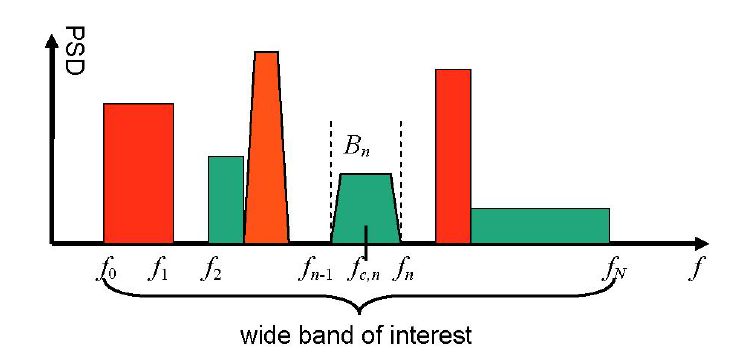
\includegraphics[height = 7 cm]{bands.png}
\caption{A digram of the Spectrum Sensing model \cite{Tian}}
\label{widebandspectra}
\end{figure*}

\subsection{Classical Sensing}
Classically, for perfect signal reconstruction, we must sample a signal such that the sampling rate must be at least twice the maximum frequency in the bandlimited signal. The continuous time signal can then be recovered using an appropriate reconstruction filter (e.g. a sinc filter). For example, we can represent a sampled continuous signal as a multiplication of the signal with a train of Dirac delta functions at multiples of the sampling period T.
%
\begin{equation}
x\left(nT\right) = \Sh\left(t-nT\right)x\left(t\right)
\end{equation}
%
where
%
\begin{equation}
\Sh\left(t-nT\right) = \sum_{k=-\infty}^{\infty} \delta\left(t - kT\right)
\end{equation}

Working the frequency domain, this multiplication becomes convolution (which is equivalent to shifting):

\begin{equation}
\hat{X}_{s}\left(f\right) = \sum_{k=-\infty}^\infty x\left(t - kT\right)
\end{equation}

Thus if the spectrum of the frequency is supported on the interval \(\left(-B, B\right)\) then sampling at intervals \(\frac{1}{2B}\) will contain enough information to reconstruct the signal \(x(\left(t\right)\). Multiplying the spectrum by a rectangle function (low-pass filtering), to remove any images caused by the periodicity of the function, and the signal \(x(\left(t\right)\) can be reconstructed from its samples:

\begin{equation}
x\left(t\right) = \sum_{n=-\infty}^\infty x\left(nT\right) sinc\left(\frac{t_nT}{T}\right)
\end{equation}

\subsection{Compressed Sensing}

However, in practice many signals encountered 'in the wild' can be fully specified by much fewer bits than required by the sampling theorem above. For example, image compression algorithms can reduce the size of a stored image to about 1\% of the size required by Nyquist sampling. If the reconstruction algorithm is able to reconstruct the image from this small amount of data, this raises the question: why collect all the data in the first place, when most of the information can be thrown away? Why not directly measure the part that will not end up being thrown away?

Compressed Sensing considers situations where the signal is \textit{undersampled} i.e. situations in which the number of samples is much smaller than the dimension of the signal (or the number of samples required by classical sampling theory). This is equivalent to a system of linear equations which is under-determined.  That is, this is a method of measuring the informative parts of a signal directly without acquiring unessential information at the same time (i.e. the parts of the signal that would be discarded in traditional compression applications). The questions then are how can we acquire these measurements in the first place, and how to 'decompress' them once they are obtained \cite{Donoho2006}. 

To answer the first, note that signals have representations in which they are sparse (i.e. the most of the co-efficients in that representation are zero, or close to zero). For example, 

\begin{enumerate}
\item  A sine wave at frequency \(\omega\) is defined as a single spike in the frequency domain yet has an infinite support in the time domain
\item An image will have values for every pixel, yet the wavelet decomposition of the image will typically only have a few non-zero coefficients
\end{enumerate} 

However, we may not be able to directly obtain those coefficients, as we may not posses an appropriate measuring device (or one may not exist). Yet we are able to measure correlations between the signal and the basis waveforms of the domain where the signal is sparse \(\phi_{k}\) i.e. 
%
\begin{equation}
y_{k} = \left\langle f \text{,} \phi_{k} \right\rangle \text{ } k = 1 \ldots m
\end{equation}
%
for \( f \in \mathbb{R}^n \) expanded in an orthonormal basis \( \psi \) s.t.
%
\begin{equation}
f(t) = \sum_{i = 1}^n x_{i}\psi_{i}(t) 
\end{equation}
%
where the \(x_{i} \) are the coefficient sequence of f. 

An example of a practical Compressive Sensing system is the single-pixel camera at Rice University \cite{Duarte2008}. Typical camera devices obtain pixel samples by exposing a bank of photon detectors (one for each pixel) to the incident light field. This data is the processed into an image.

The single pixel camera takes pictures by first directing the incoming light field onto an array of tiny mirrors (one for each pixel). Each mirror can be either be oriented towards a single photon detector, or oriented away from the detector. In this setup, a measurement is taken as the sum of all the incident light beams. Afterwards, the mirrors are flipped to a new random configuration, and another measurement is taken. This process is repeated, until enough information has been collected to reconstruct the image. Figure \ref{singlepixelcamera} shows the operation of the single pixel camera.

\begin{figure*}[h]
\centering
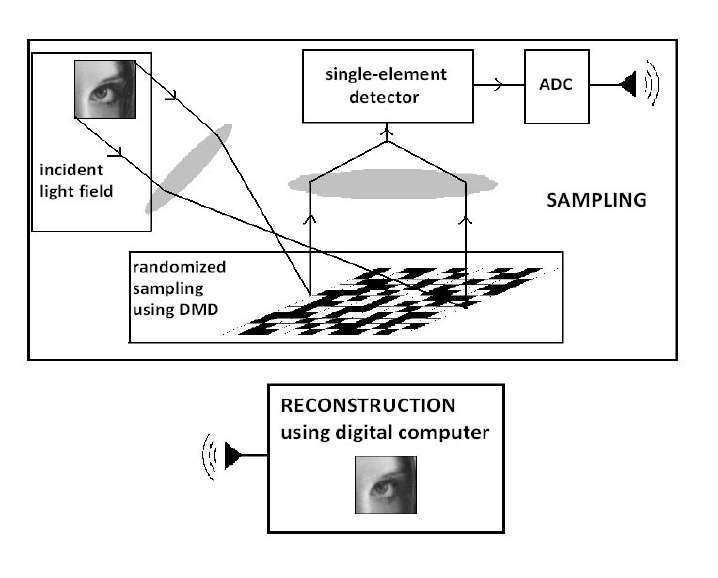
\includegraphics[height = 7 cm]{singlepixel.png}
\caption{The operation of the single pixel camera at Rice University \cite{singlepixelimaging}}
\label{singlepixelcamera}
\end{figure*}

%Compressive Sensing works best if the \(x_{i}\) are compressible (i.e. they are distributed according to a power law), and the error \(\|x - x_{s}\|\) is small.

%In Compressive Sensing measurements are taken is an incoherent basis, as opposed to the basis of the original signal. 

The question all this raises is where do we do our sensing? In other words, given that we know a basis in which our signal is sparse, \(\phi\), how do we choose \(\psi\)? It's best to choose \(\psi\) so that the signal is 'spread out' relative to the signal's expansion in \(\phi\). Such pairs are said to be incoherent. 

\begin{defn}
A pair of bases is said to be incoherent if the largest projection of two elements between the sensing (\(\psi\)) and representation (\(\phi\)) basis  is in the set \( [1 , \sqrt{n}] \), where \( n \) is the dimension of the signal. The coherence of a pair of bases is denoted by \(\mu\).
\end{defn}

This implies that sensing with incoherent systems is good (in the sine wave example above it would be better to sample randomly in the time domain as opposed to the frequency domain), and efficient mechanisms ought to acquire correlations with random waveforms (e.g. white noise).

\textbf{Theorem} \cite{Candes2006}
Fix f \(\in \mathbb{R}^n\) with a sparse coefficient basis, \(x_{i}\) in \(\psi\). Then a reconstruction from \(m\) random measurements in \(\phi\) is possible with probability \(1 - \delta\) if: 

\begin{equation}
m \geq C \mu^2(\phi, \psi) S \log\left(\frac{n}{\delta}\right)
\end{equation}
\label{minsamples}

where \( \mu(\phi, \psi)\) is the coherence of the two bases, and \(S\) is the number of non-zero entries on the support of the signal.

Then \(f*\) (the proposed reconstruction) is given by \(f^* = \psi x^*\) where \(x^*\) is the solutionn to the convex optimisation program (n.b. \(\| x\|_{l_{1}} := \sum_{i} |x_{i}| \)):

\begin{equation}
min\|\tilde{x}\|_{l_{1}} \text{ subject to } y_{k} = \left\langle \phi_{k} \text{,} \psi x^* \right\rangle \text{   } \forall k \in M \subset [1 \ldots n]
\end{equation}
\label{program0}

i.e. \textbf{CS: Sample non-adaptively in an incoherent domain and invoke linear programming after the acquisition step}

Thus the role of \(l_{1}\) minimisation is to decompress the data. There are many ways to perform this operation: some popular methods are basis pursuit \cite{Chen1998} and Greedy approaches such as Orthogonal Matching Pursuit \cite{Tropp2007}. 

It may be remarked that the \(l_0\) norm:
%
\begin{equation}
\vectornorm{l_0} = \{\# i, x_i \neq 0\}
\end{equation}
%
is a more appropriate functional to minimise. In fact under this norm, \(m \geq 2k\) measurements will suffice to uniquely determine all \(k\)-sparse signals. However, this norm is not convex and so minimising it is an NP-hard problem. As we are seeking sparse solutions the \(l_1\)-norm will suffice \cite{Donoho2006a}. This is because all vectors in a random \(k\)-dimensional subspace of an \(n\)-dimensional space are approximately Gaussian (in the sense that the components are distributed according to an approximate normal distribution). Such vectors have roughly equivalent norms, and so any solution to the \(l_1\) minimisation problem will be the same solution to the \(l_1\) minimisation problem for sufficiently sparse signals.

\subsubsection{Incoherence, isometries and all that}
To recover a sparse vector, we must make sure that the vectors are not in the null space of the sensing matrix (otherwise there would be no hope of recovery). We also require that any subset of \(S\) columns taken from the measurement matrix be nearly orthogonal w.r.t sparse vectors: i.e. all pairwise distances between S-sparse vecotrs be well preserved in the measurement space.

This can be summed up in the following inequality (Restricted Isometry Property) \cite{Emma}:


\begin{definition}[Restricted Isometry Property]
\begin{equation}
\left(1-\delta\right)\vectornorm{x}_{l_2}^2 \leq \vectornorm{Ax}_{l_2}^2 \leq \left(1+\delta\right) \vectornorm{x}_{l_2}^2
\end{equation}
\label{RIP}
\end{definition}


We are also in a position to evaluate the meaning of the constant \(\mu\) in \ref{minsamples}. We are considering sampling within orthonormal systems (for example, Time and Frequency):
%
\begin{equation}
A*A = nI
\end{equation}
\label{orthonormal}
%
so that each row or column has \(l_2\) norm equal to \(sqrt{n}\). \(A\) is any matrix satisfying this property (examples include the Fourier matrix and the Dirac matrix). Thus \(\mu\) must be in the set \(\left[1, \sqrt{n}\right]\). \(\mu\) then, is a measure of how concentrated the rows of our measurement matrix is - i.e. how much information is spread across each vector. If \(\mu = 1\) then the rows are 'flat' -  and we need relatively fewer samples to reconstruct an S-sparse signal (i.e. each sample provides the same amount of information). However, if the rows contain all non-zero entries except for a single component, then \(\mu^2 = n\) and we will need to observe all components to determine the non-zero one (i.e. we have no guarantees of recovery from limited samples) \cite{Candes2007}. 

Noting that the measurements we take are projections from our orthonormal system (from example time) onto a sparsifying basis (i.e. frequency) we can see that:

\begin{equation}
\mu = max_{k,j} |\langle \phi_k, \psi_j \rangle |
\end{equation}
\label {mudef}
 
So we need to choose a sensing basis, where the vectors will be 'spread out', and the degree of spreading is characterised by \(\mu\).

\subsubsection{Short, Fat matrices}
As remarked upon earlier: Compressive Sensing is equivalent to solving an under-determined linear system, with the constraint that we seek the sparsest solution. The content of the previous sections amounts to constraints on the number of rows of matrix of this linear system. 

If we had an Oracle which could tell us where the non-zero components of our solution were, then we would need only as many rows of the matrix as there were non-zero components in the signal to fully specify the problem. 

%\begin{figure*}[h]
%\centering
%\includegraphics[height = 7 cm, width=\textwidth]%{compressive_sensing_example.jpg}
%\caption{A visualisation of the Compressive Sensing problem as an under-%determined system}
%\label{l1l2}
%\end{figure*}

However, such and Oracle does not exist, and so we're left with the task of constructing a matrix to recover those components. Knowing that we're looking for k-sparse solutions, we need a matrix with at least 2k columns which are linearly independent. Equivalently, all images of \(k\)-sparse vectors under the operation of the sensing matrix \(\Phi\) must be distinct. From this, any k-sparse signal can be reconstructed from \(Ax\). 

To prove this assume the opposite - then there are two vectors \(x, x' \in \mathbb{R}^n\) such that \(Ax = Ax'\). I.e. \(A(x-x') = 0\). However, \((x-x')\) is 2k-sparse and so there is a linear dependence between 2k columns of the sensing matrix A. We have a contradiction, and so 2k columns will suffice to reconstruct a k-sparse signal. 

The problem with this is that we are trying to find the support of a k-sparse signal over a vector of length N, and so we would need to check all \(N \choose k\) combinations of k-sparse signals which is prohibitively computationally expensive. Is there some way to gain the advantages of sparsity, without having to minimise a non-convex functional?

As it turns out, the answer is yes. If we take \( m \geq C \mu^2(\phi, \psi) S \log\left(n\right) \) rows minimising the \(l_{1}\) norm will find the sparsest solution. This is because the \(l_1\) norm is an octahedron (in 3-dimensions, in higher dimensions it has an analogous spiky geometry), and solutions are more likely to intersect the norm at the points. Figure \ref{l1l2} shows this.

\begin{figure*}[h]
\centering
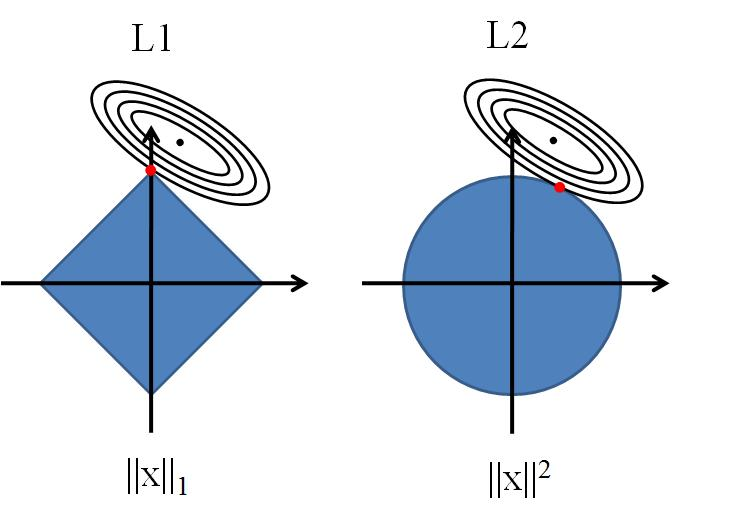
\includegraphics[height = 7 cm]{l1l2.jpg}
\caption{Solutions to the Compressive Sensing optimisation problem intersect the \(l_1\) norm the points where all components (but one) of the vector are zero (i.e. it is sparsity promoting) \cite{Tibshirani1996}}
\label{l1l2}
\end{figure*}

\subsubsection{Bayesian Compressive Sensing}
Based on the discussion above we can represent the compressive sensing measurements as: 

\begin{equation}
\textbf{g} = \Phi	\textbf{w}
\end{equation}

where \(\Phi\) is a \(K \times	N\) matrix which is the product of the measurement and sparse bases described earlier.

Note that the measurements may be noisy, with the measurement noise represented by a zero mean Gaussian distribution and unknown variance \( \sigma^2 \):

\begin{equation}
\textbf{g} = \Phi \textbf{w} + \textbf{n}
\end{equation}
\label{CSequation}

Where \textbf{n} is the vector representing the vector of noise, and has the same support as the measurements. 

Previous sections have shown how the weights \(w\) may be found through optimisation methods such as basis pursuit or greedy algorithms. Here, an alternative Bayesian model is described.

From \ref{CSequation} we have a Gaussian likelihood model: 

\begin{equation}
p \left( \textbf{g} \mid \textbf{w}\text{,} \sigma^2 \right) = (2 \pi \sigma^2)^{-K/2} \exp{\left(- \frac{1}{2 \sigma^2} \|\textbf{g} - \Phi	\textbf{w}\|_{2}^{2} \right)} 
\end{equation}

The above has converted the CS problem of inverting sparse weight \textbf{w} into a linear regression problem with a constraint (prior) that \textbf{w} is sparse. 

To seek the full posterior distribution over \textbf{w} and \( \sigma^2 \), we can chose a sparsity promoting prior. A popular sparseness prior is the Laplace density functions:

\begin{equation}
p\left(w\mid\lambda\right) = \left(\frac{\lambda}{2}\right)^N exp{-\lambda \sum_{i=1}^{N} |w_i|}
\end{equation}

Note that the solution the convex optimisation problem \ref{program0} corresponds to a maximum \textit{a posteriori} estimate for \(w\) using this prior. I.e this prior is equivalent to using the \(l_1\) norm as an optimisation function (see figure \ref{laplacenormal} \cite{Tibshirani1996}).

\begin{figure*}[h]
\centering
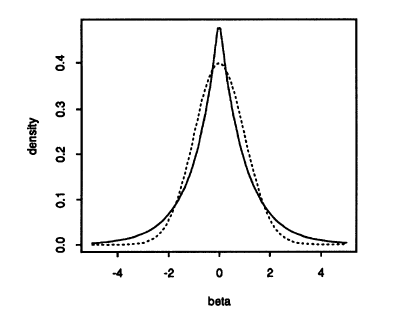
\includegraphics[height = 7 cm]{LaplaceandNormalDensity.png}
\caption{The Laplace (\(l_1\)-norm, bold line) and Normal (\(l_2\)-norm, dotted line) densities. Note that the Laplace density is sparsity promoting as it penalises solutions away from zero more than the Gaussian density. \cite{Tibshirani1996}}
\label{laplacenormal}
\end{figure*}

The full posterior distribution on \(w\) and \(\sigma^2\) may be realised, by using a hierarchical prior instead. To do this, define a zero-mean Gaussian prior on each element of \(w\):
%
\begin{equation}
p\left(w\mid a\right) = \prod_{i=1}^{N}\mathbb{N}\left(w_i\mid 0, \alpha_{i}^-1\right)
\end{equation}
%
where \(\alpha\) is the precision of the distribution. A gamma prior is then imposed on \(\alpha\):

\begin{equation}
p\left(\alpha \mid a, b \right) = \prod_{i=1}^{N} \Gamma\left( \alpha_i \mid a, b \right)
\end{equation}

The overall prior is found by marginalising over the hyperparameters:

\begin{equation}
p\left( w \mid a, b \right) = \prod_{i=1}^{N} \int_{0}^{\infty} \mathbb{N}\left(w_i\mid 0, \alpha_{i}^-1\right) \Gamma\left( \alpha_i \mid a, b \right)
\end{equation}

This integral can be done analytically and is a Student-t distribution. Choosing the parameters \(a,b\) appropriately we can make the Student-t distribution peak strongly around \(w_i = 0\) i.e. sparsifying. This process can be repeated for the noise variance \(\sigma^2\). The hierarchical model for this process is shown in \ref{bayesiancs}. This model, and other CS models which not necessarily have closed form solutions, can be solved via belief-propagation \cite{Baron2010}

\begin{figure*}[h]
\centering
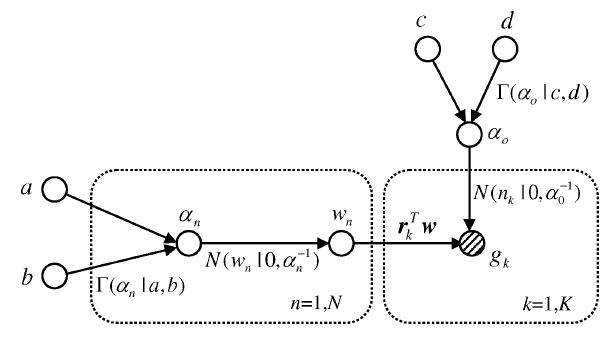
\includegraphics[height = 7 cm]{bayesiancs.png}
\caption{The hierarchical model for the Bayesian CS formulation \cite{Ji2008}}
\label{bayesiancs}
\end{figure*}